

We now present three topics of discussion before making our concluding remarks. 

\subsection{I-priors vs. g-priors}
\label{sec:gprior}

In the Bayesian variable selection literature, the g-prior based off \cite{Zellner1986} is a popular objective choice for an uninformative prior on $\boldsymbol\beta$. We have some thoughts on the instances where g-prior would be better suited than the I-prior. The g-prior on the coefficients of a linear model in \eqref{eq:linmod1} is defined as
\[
	\boldsymbol\beta \sim \text{N}(\boldsymbol\beta_0, g(\psi\mathbf X^\top \mathbf X)^{-1})
\]
where $g$ is a constant which is either fixed or a parameter to be estimated. The usual choice for $\boldsymbol\beta_0$ would be $\mathbf 0$, especially after centering the data. In essence, the covariance matrix is equal to the (scaled) inverse Fisher information. This is certainly the opposite of the intuition behind  I-priors: For g-priors, should there be much Fisher information about the parameters, the prior covariance would be \textit{small}, and thus the prior would be concentrated around zero.

\cite{Bergsma2014} notes the following interpretation of g-priors: the g-prior is equivalent to an I-prior on $\boldsymbol\beta$ if the Euclidean distance used to calculate the Fisher information is instead replaced by the Mahalanobis distance. That is, 
\[
	I_{\text{Mah}}[\boldsymbol\beta] = (\psi\mathbf X^\top \mathbf X)^{-1}
\]
where the Mahalanobis distance is given as $||\mathbf x||^2_{\text{Mah}} = \mathbf x^\top (\psi\mathbf X^\top \mathbf X)^{-1} \mathbf x$. The use of a Mahalanobis-type metric results in distances between vectors to be invariant to linear transformations. This helps in interpretation somewhat - if we have two variables which are measured on incomparable scales, such as height and weight, then the Euclidean distance between height and weight does not make sense, but the Mahalanobis distance does. Thus a g-prior may be sensible in such situations. If however we have variables measured on the same scale, such as repeated measures of a variable over time, then the I-prior, whose Fisher information is based on the Euclidean distance, is sensible to be used. However, the difference between I-priors and g-priors, looking at it from this point of view, merely helps from an interpretability standpoint. 

What matters perhaps is how we can take advantage of the covariance/correlation structure in the data to influence our prior and hence posterior. Proponents of g-priors argue that the g-prior serves this purpose: ``\textit{...use of $\propto (\mathbf X^\top\mathbf X)^{-1}$ tends to replicate design correlation}'' \citep{George1993}; ``\textit{The choice of $(\mathbf X^\top\mathbf X)^{-1}$ serves to replicate the covariance structure of the likelihood...}'' \citep{Chipman2008}. What we can see is that the linear model in \eqref{eq:linmod1} with centred variables equipped with the g-prior, i.e.
\begin{align}
	\begin{gathered}
		\mathbf y = \boldsymbol\alpha + \mathbf X \boldsymbol\beta + \boldsymbol\epsilon \\
        \boldsymbol\epsilon \sim \text{N}(\mathbf 0, \psi^{-1}\mathbf I_n) \\
        \boldsymbol\beta \sim \text{N}\big(\mathbf 0, g(\mathbf X^\top\mathbf X)^{-1}\big)
	\end{gathered}
\end{align}
is equivalent to the model with an independent covariance structure in the prior, with the transformation $\tilde{\mathbf X} = \mathbf X(\mathbf X^\top\mathbf X)^{-1/2}$ and $\tilde{\boldsymbol\beta} = (\mathbf X^\top\mathbf X)^{1/2}\boldsymbol\beta$, given by
\begin{align}
	\begin{gathered}
		\mathbf y = \boldsymbol\alpha + \tilde{\mathbf X} \tilde{\boldsymbol\beta} + \boldsymbol\epsilon \\
        \boldsymbol\epsilon \sim \text{N}(\mathbf 0, \psi^{-1}\mathbf I_n) \\
        \tilde{\boldsymbol\beta} \sim \text{N}(\mathbf 0, g^2 \mathbf I)
	\end{gathered}
\end{align}
The transformation done onto the $\mathbf X$ variables is a type of whitening transformation\footnotemark, with the $(\mathbf X^\top\mathbf X)^{-1/2}$ known for being a decorrelating matrix. The I-prior on the other hand does not achieve this transformational decorrelating equivalence and perhaps is better at capturing the covariance/correlation structure in the data. The simulation study that we have done with the g-prior seem to give results similar to using independent priors for $\boldsymbol\beta$, like the SSVS, KM and GVS methods.

\footnotetext{Check that the sample covariance for $\tilde{\mathbf X}$ is the identity matrix.}

\begin{figure}[h]
	\centering
	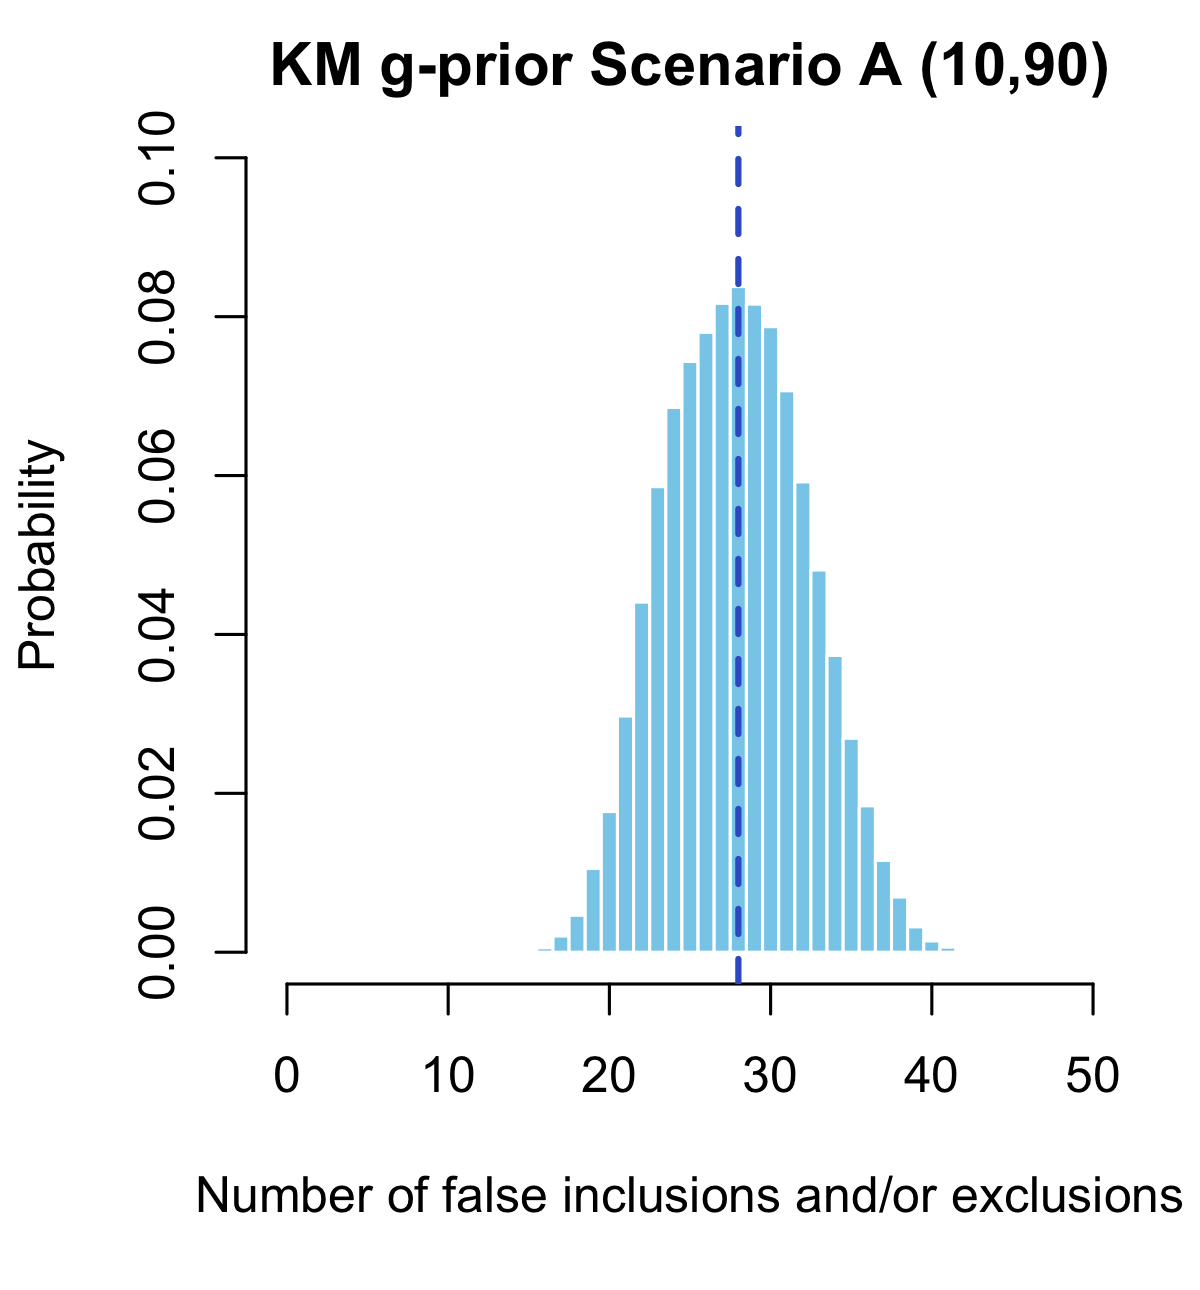
\includegraphics[height=2.1in]{figure/Ag} \hspace{-4mm}
	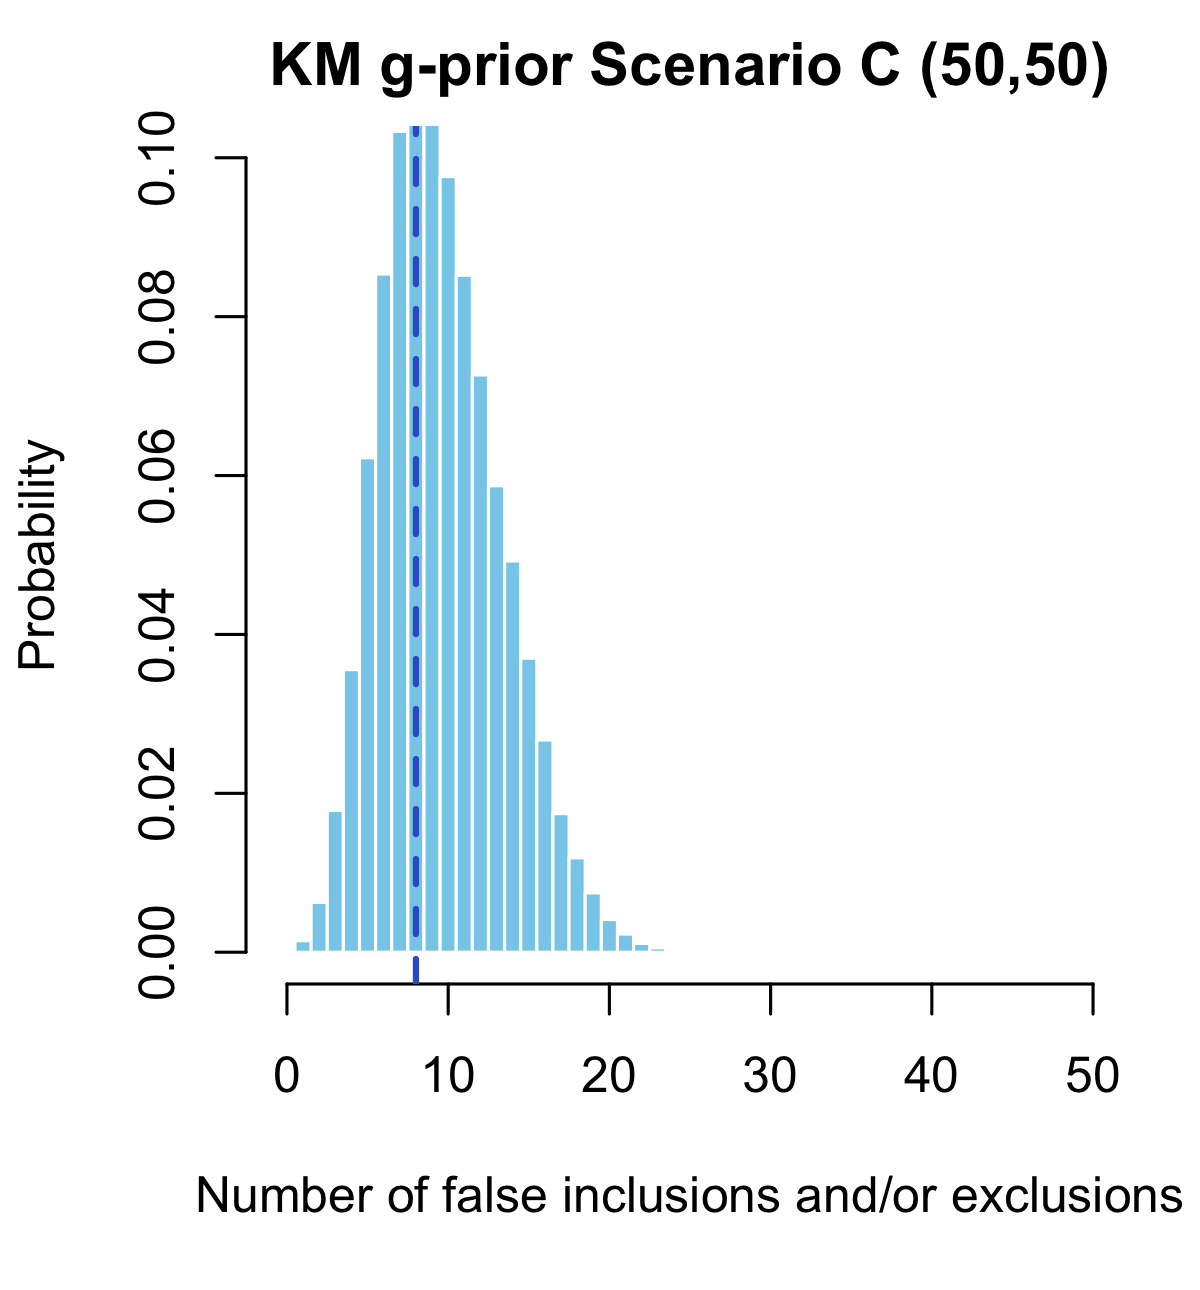
\includegraphics[height=2.1in]{figure/Cg} \hspace{-4mm}
	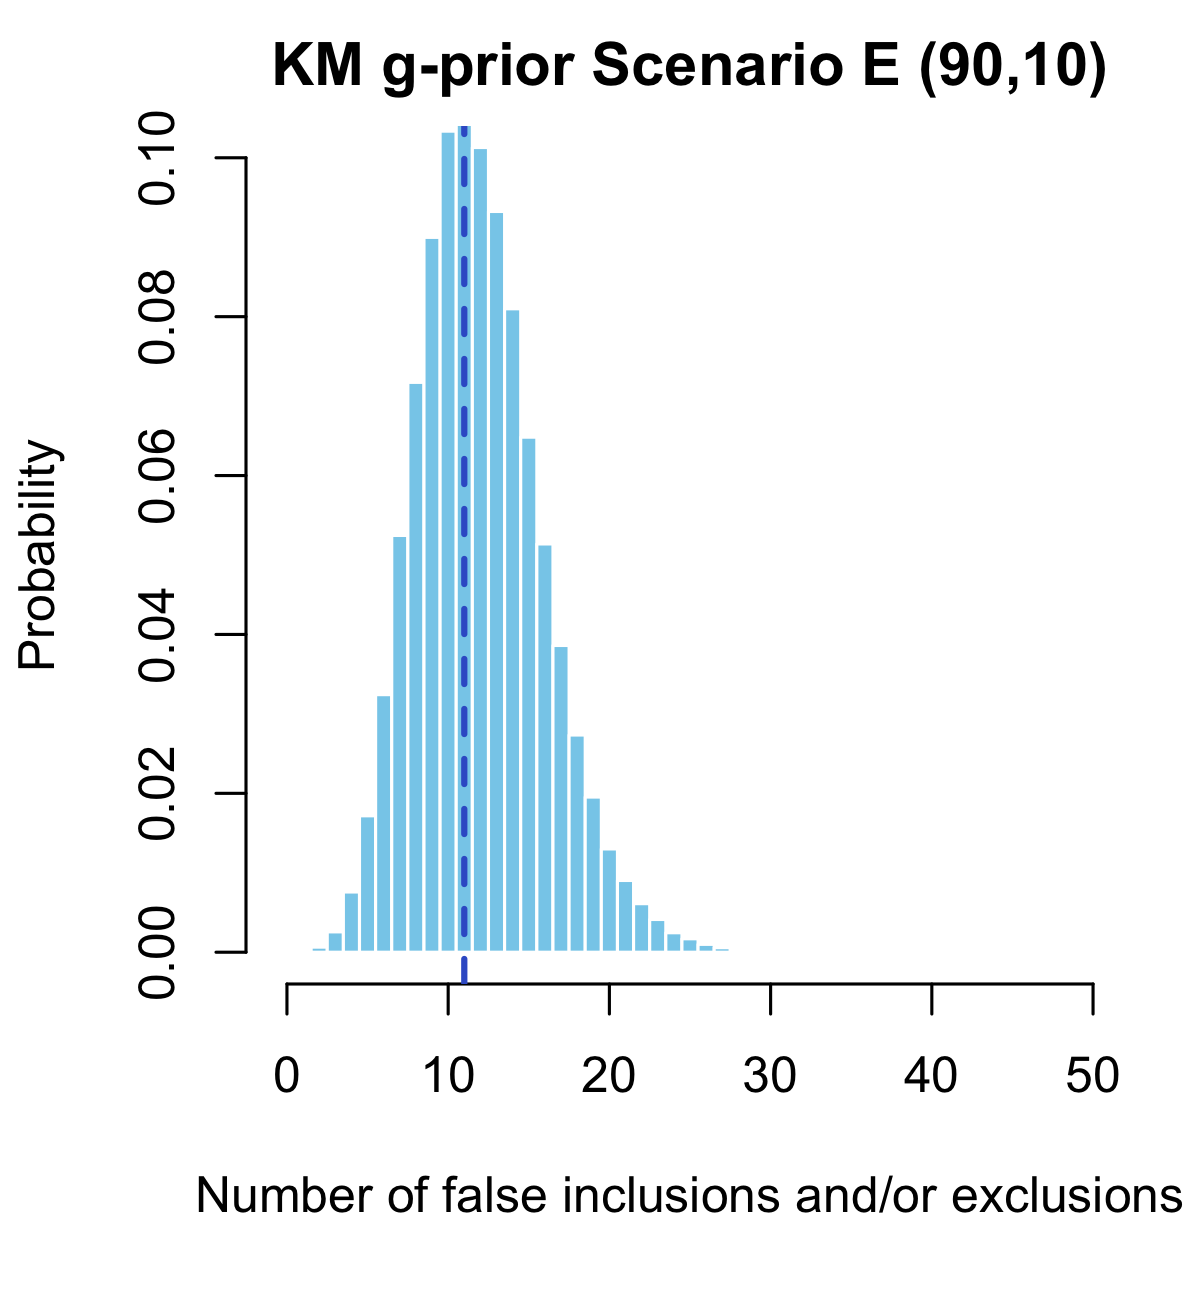
\includegraphics[height=2.1in]{figure/Eg}
	\label{fig:gpriorsim}
	\caption{Repeat of the simulation experiment seen earlier but this time using g-priors. The results show that the g-prior does not produce good results across all scenarios, as there is rarely very few false inclusions and/or exclusions.}
\end{figure}

\vspace{-2mm}
\subsection{The \texorpdfstring{$p > n$}{p > n} case}
\vspace{-2mm}

In the original I-prior modelling methodology, models whose regression function lives in a high- or possibly infinite- dimensional RKHS $\mathcal F$ are able to be dealt with by considering only a smaller dimensional sub-space of $\mathcal F$ (whose dimension is at most $n$), effectively reducing dimensionality of the problem when $p>n$. Specifically, what we did was decompose the RKHS $\mathcal F$ into $\mathcal F_n + \mathcal R$ where $\mathcal F_n \perp \mathcal R$. By considering only functions in this smaller subspace $\mathcal F_n \subset \mathcal F$, we are able to use the Fisher information which is guaranteed to exist for functions in $\mathcal F_n$ and apply the I-prior methodology. For the remaining space $\mathcal R$, we have no Fisher information and we resort to a prior guess for functions in this space if we are unable to obtain more data.

\stepcounter{todocounter}
\todo[caption={\thetodocounter. Actually, data is insufficient in $p>n$ case to determine which model should be selected. Not sure of I-prior suitable in these cases.}]{Worth exploring?}
While the original I-prior modelling gives promising regression results in the $p>n$ case, sadly our simulation study shows that this promise does not transfer to the Bayesian variable selection application. In fact, the results deteriorate as soon as a simulation with $n=p-1$ is run. The reasons for this might be two-fold. Firstly, following the argument in the above paragraph, Fisher information only exists for at most $n < p$ number of $\boldsymbol{\beta}$s, and thus the remaining $(p-n)$ $\boldsymbol{\beta}$s do not make use of this objective I-prior, but instead must be supplemented with some other prior, which is possibly subjective. Secondly, we think the reason also lies in the Gibbs sampling procedure, where the inverse of $\mathbf X^\top\mathbf X$ needs to be calculated. This is not possible as it is singular in the $p>n$ case. A $p$-variate normal distribution with a singular covariance matrix, like the I-prior for $\boldsymbol{\beta}$ in the case of $p>n$, will only have a probability distribution defined on a lower dimensional subspace. Perhaps the first and second reasoning are related, and to put it simply, there just isn't enough information to go around.

Further research into this issue is ongoing. The key may lie in projecting the regression/variable selection problem into a lower dimension without losing much of the information in the original dimension. One of the methods explored was Bayesian factor regression (the Bayesian analogue of principle components regression - see \citealp{West2003}). It involves the reduced singular value decomposition (SVD) of our data $\mathbf X=\mathbf F \mathbf A$, where $\mathbf F$ is the $n \times k$ factor matrix and $\mathbf A$ is the $k \times p$ matrix of loadings satisfying $\mathbf A\mathbf A^\top  = \mathbf I_k$ and $\mathbf F^\top \mathbf F = \mathbf D^2$, a diagonal matrix of the $k$ positive singular values\footnotemark. Substituting the reduced SVD into the regression equation we obtain
\begin{align*}
	 \mathbf y &= \boldsymbol{\alpha} 
	 + {\color{gray} \overbrace{\phantom{i}}^{\mathbf X} \hspace{-6.8mm} {\color{black} \mathbf F } \hspace{-0.5mm}
     \underbrace{{\color{black} \mathbf A \, \boldsymbol\beta}}_{\boldsymbol\theta} }
     + \ \boldsymbol{\epsilon},
\end{align*}
where $\boldsymbol{\theta}$ is the $k$-vector of regression parameters of the responses against the factors as explanatory variables. The Bayesian solution would involve setting priors on $\boldsymbol{\theta}$ and the other parameters of the model, and estimating the model using MCMC methods. Inference on the original parameters $\boldsymbol{\beta}$ is then made possible via the mapping $\mathbf A^\top\boldsymbol{\theta} \mapsto \boldsymbol{\beta}$ (actually, $\boldsymbol{\theta} \mapsto \mathbf A\boldsymbol{\beta}$ is a many-to-one map, so multiple generalized inverses $\boldsymbol{\beta} = \mathbf A^\top\boldsymbol{\theta} + \mathbf b$ exist $\forall b \in \mathbb R^p$ such that $\mathbf A\mathbf b = \mathbf 0$, and the canonical choice is the standard ``least-norm'' inverse based on $\mathbf b = \mathbf 0$).

\footnotetext{The full principle components decomposition of $\mathbf X$ is given as $\mathbf F = \mathbf X \mathbf W$, where  $\mathbf W$ is a $p \times p$ matrix whose columns are the eigenvectors of $\mathbf X^\top\mathbf X$, also known as the loadings. $\mathbf F$ is known as the factor or score matrix. 

The full SVD of $\mathbf X$ is $\mathbf X = \mathbf U \mathbf D \mathbf W^\top$, with $\mathbf U\mathbf U^\top = \mathbf I_n$, $\mathbf W\mathbf W^\top = \mathbf I_p$, and $\mathbf D$ being an $n\times p$ diagonal matrix of positive reals called the singular values of $\mathbf X$. Consider $\mathbf X^\top\mathbf X = \mathbf W \mathbf D \mathbf U^\top\mathbf U \mathbf D \mathbf W^\top = \mathbf W \mathbf D^2 \mathbf W^\top$. By comparison, the matrix $\mathbf W$ is equivalent to the eigenvectors of $\mathbf X^\top\mathbf X$, and the singular values $\mathbf D_{ii}$ are equivalent to the positive roots of the eigenvalues of $\mathbf X^\top\mathbf X$. 

Moreover, $\mathbf F = \mathbf X \mathbf W = \mathbf U \mathbf D \mathbf W^\top\mathbf W = \mathbf U \mathbf D$, thus establishing the connection between principle components and SVD, $\mathbf X = \mathbf F\mathbf W$. For dimension reduction, only the first $k < p$ principle components/singular values of $\mathbf X$ are considered (i.e. $\mathbf A$ is a truncated version of $\mathbf W$ by considering only the first $k$ columns), which is what we have done here.}

Bayesian factor regression is a promising route, but in our variable selection model there is  an issue. Our original parameters are actually $\boldsymbol{\beta}_{\boldsymbol{\gamma}} = \boldsymbol{\beta}\cdot\boldsymbol{\gamma}$, and when these are projected onto a lower-dimensional space of parameters $\boldsymbol{\theta}$ and the regression model gives estimates for $\boldsymbol{\theta}$, there is no way of recovering back the indicator variables $\boldsymbol{\gamma}$ to say which of the variables $\mathbf X$ should be kept or deleted. In Bayesian factor regression, the priors are set for $\boldsymbol{\theta}$ rather than $\boldsymbol{\beta}$, so applying the I-prior certainly requires some additional thought as well.

\subsection{The logistic variable selection model}

\stepcounter{todocounter}
\todo[caption={\thetodocounter. For future direction, look specifically into binary outcome models. GLM may be too broad.}]{Concentrate first on logistic}
We are able to extend the Bayesian variable selection to the logistic model, and by extension to the generalised linear models, just as \cite{Kuo1998} have done (our I-prior model is basically their model equipped with an I-prior). The logistic I-prior variable selection model is
\begin{align}
	\begin{gathered}
		y_i \sim \text{Bern}(\pi_i) \\
        \logit(\pi_i) = \alpha + \gamma_1\beta_1 x_{i1} + \cdots + \gamma_p\beta_p x_{ip} \\
        i=1,\dots,n.
	\end{gathered}
\end{align}
The Fisher information for the coefficients $\boldsymbol\beta$ in the logistic regression is
\[
	I[\boldsymbol\beta] = \mathbf X^\top \mathbf W \mathbf X,
\]
where $\mathbf W = \text{diag}[\pi_1(1-\pi_1), \dots, \pi_n(1-\pi_n)]$. An I-prior on $\boldsymbol\beta$ would then be
\[
	\boldsymbol\beta \sim \text{N}(\mathbf 0, \boldsymbol\Lambda\mathbf X^\top \mathbf W \mathbf X\boldsymbol\Lambda).
\]
To complete the model specification we also assign priors on $\boldsymbol{\gamma}$, $\alpha$ and possibly $\boldsymbol{\lambda}$ if these are to be estimated as well.

\begin{figure}[h]
	\centering
	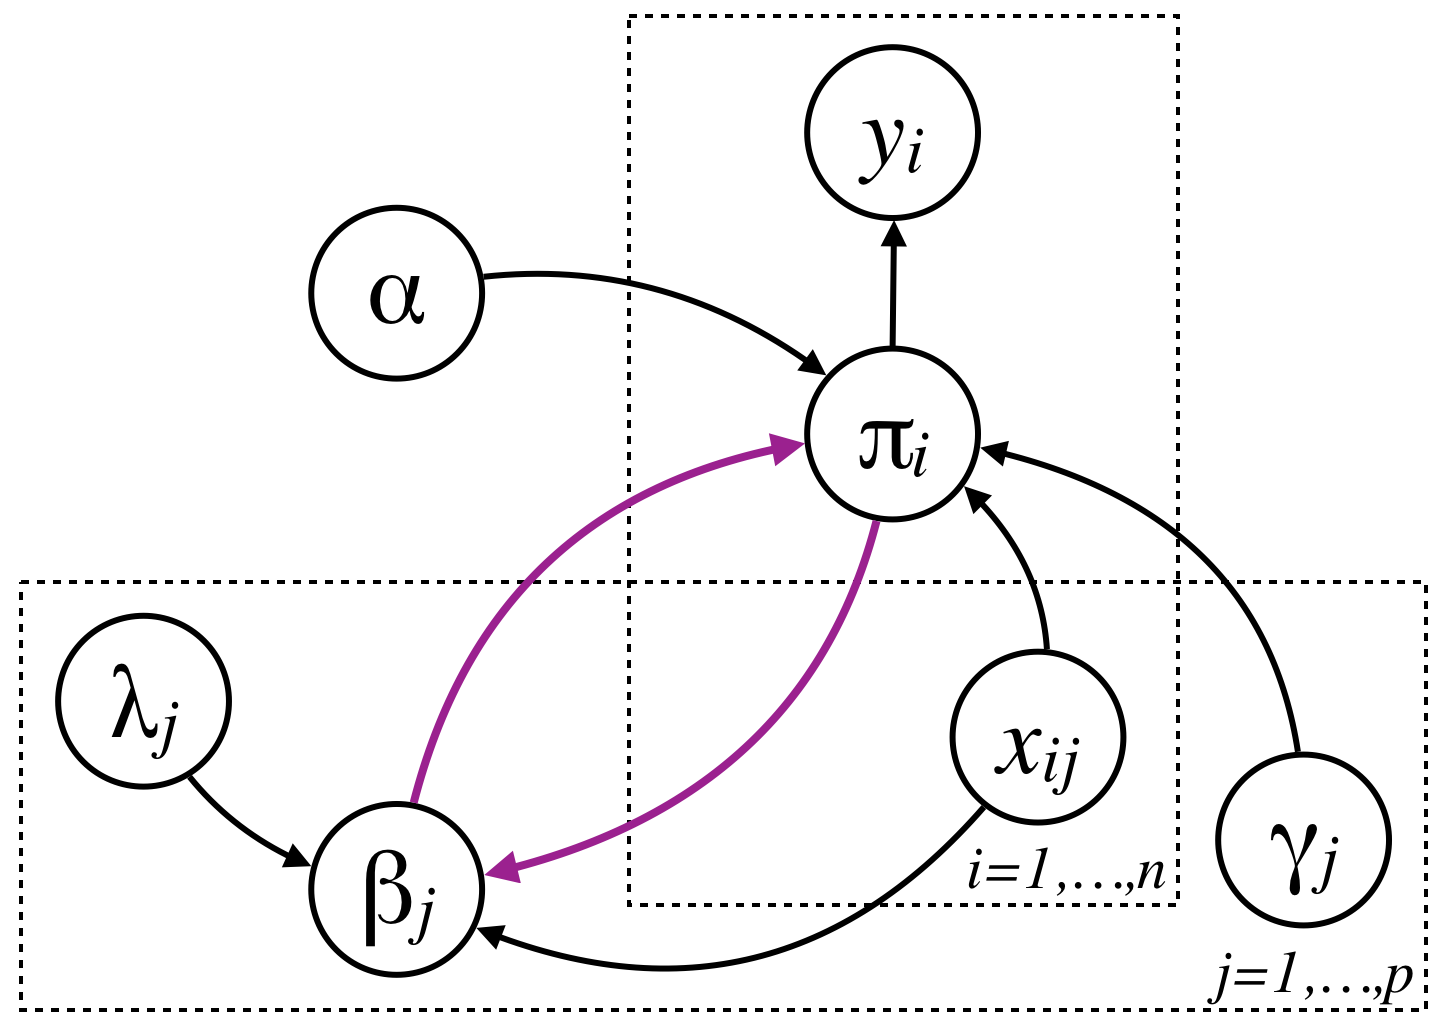
\includegraphics[height=2.4in]{figure/logistic-iprior}
	\label{fig:logipriordep}
	\caption{Graphical representation of the I-prior logistic model. There is a double dependence between the prior $\boldsymbol\beta$ and the parameters $\boldsymbol{\pi}$ as shown by the purple edges.}
\end{figure}

There is a problem, in that the estimation of the $\pi_i$s has a double dependence on the parameters $\boldsymbol\beta$, as shown in Figure \ref{fig:logipriordep}. Specifying the $\pi_i$s a priori instead of estimating them avoids the reuse of data in the prior, and thus simplifies matters greatly. Following \cite{Ntzoufras2008} in his specification of a g-prior for a GLM and in the absence of information, we can put $\pi_1=\dots=\pi_n = 1/2$ to indicate our indifference. The I-prior then becomes
\[
\boldsymbol\beta \sim \text{N}\left(\mathbf 0, \frac{1}{4}\boldsymbol\Lambda\mathbf X^\top \mathbf X\boldsymbol\Lambda\right).
\]

\stepcounter{todocounter}
\todo[caption={\thetodocounter. Try probit link instead of logit link.}]{Try probit}
\stepcounter{todocounter}
\todo[caption={\thetodocounter. Try latent variable model representation of probit model.}]{Try latent variables}
A simulation study was carried out to see how well the I-prior performs in logistic regression variable selection for differing values of $p$, the number of covariates, while sample size was help constant at $n=200$. The covariates were simulated using the same procedure as in the previous simulation study, but the response variables were sampled from Bernoulli distributions with probabilities corresponding to the linear predictor with a logit link function. The number of zeros in the true value of $\boldsymbol{\beta}$ was kept to be roughly 10\% of the value of $p$, e.g. $p=5$ has 1 zero, $p=50$ has 5 zeros, and so on. We found that the I-prior method works very well for small values of $p$, but progressively worsens as $p$ gets larger. For cases with few variables to select from, the results often mirrored the GLM fit using Fisher scoring algorithm - in that the variables that were deleted coincided with the ones not found to be statistically significant\footnotemark. The variable selection method was intended really for large models, such that the evaluation of each possible model one by one would be impractical. \stepcounter{todocounter}\todo[caption={\thetodocounter. Try varying values of the $\beta$s (instead of just zeros and ones) to increase signal-to-noise ratio.}]{Try varying the $\beta$s} In this regard, it is a shame that the I-prior does not perform as well as it did in the linear case (see Figure \ref{fig:logsimiprior}).

\footnotetext{It was noted that past a certain value of $p$, the ``perfect separation'' phenomenon occurred often, where some covariates are found to not give any variability to the responses. In these situations, convergence of the GLM fails and any inference on the significance of the regression coefficients are unreliable.}

\begin{figure}[h]
	\centering
	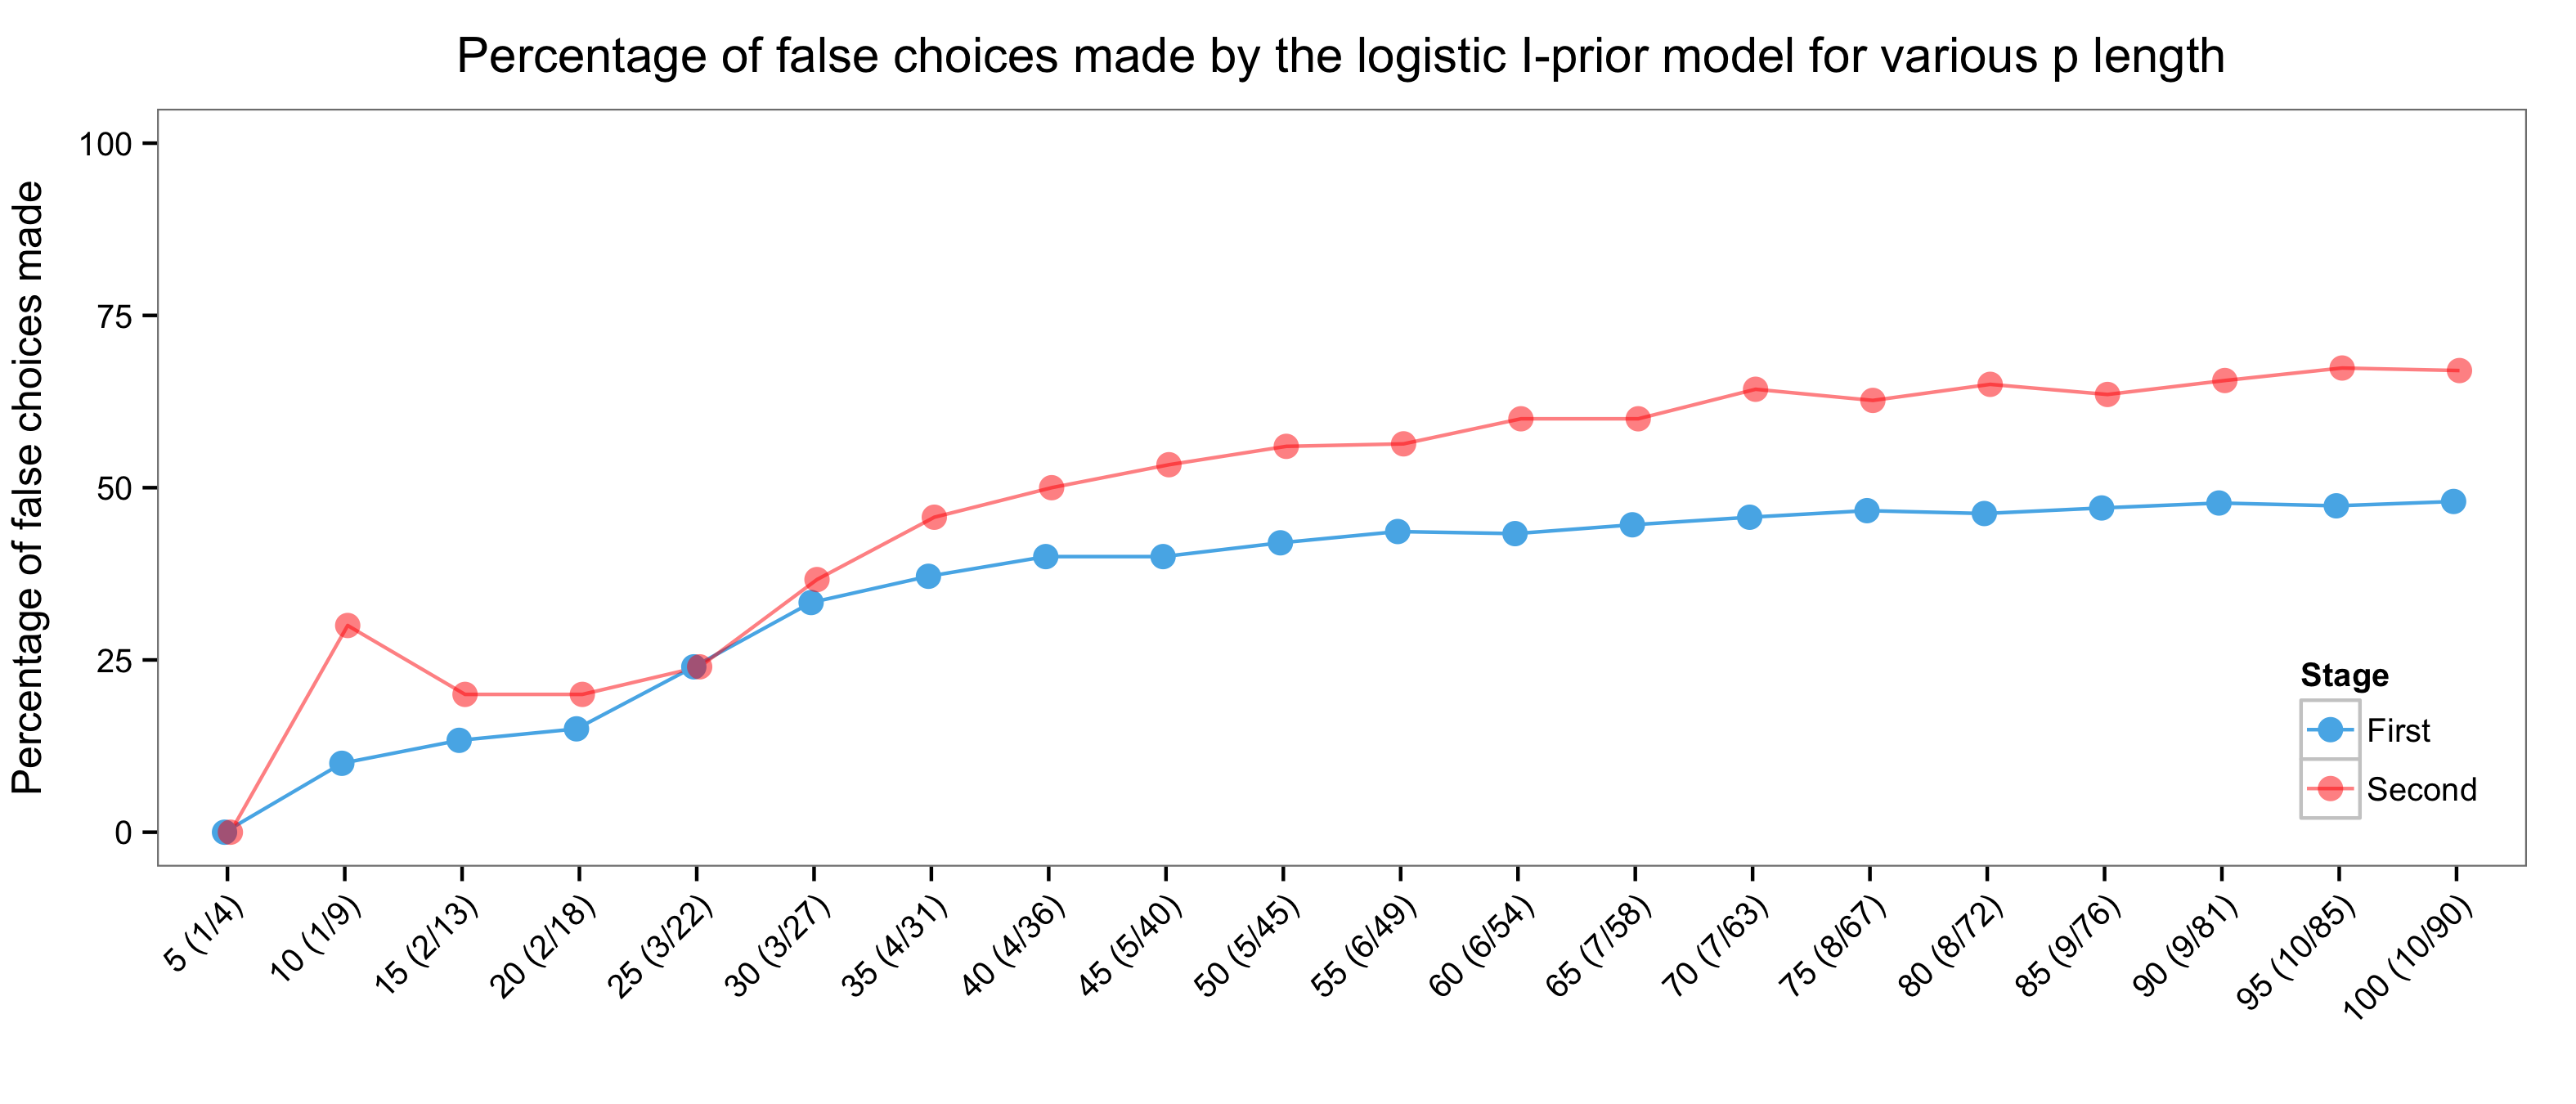
\includegraphics[width=5.8in]{figure/logsimiprior} \vspace{-7.5mm} 
	\caption{A plot showing the amount of false choices that the I-prior method made across varying $p$. For each scenario, $10,000$ MCMC samples were obtained and the experiment repeated 10 times, with the statistic of interest being the number of false choices each of these $10,000 \times 10$ models had. The points in the graph indicate the mode for the number of false choices the I-prior made for each scenario as a percentage of the total number of variables. It can be seen that false choices are low when $p$ is low, and performance progressively worsens as $p$ increases. Also note that the two-stage procedure fails to bring the improvement that was seen in the linear case. \label{fig:logsimiprior}}
\end{figure}
 